\documentclass{beamer}

\AtBeginDocument{\newcommand{\im}{\textnormal{i}}}

% Tema da apresentação
\usetheme{Madrid} % Outros temas: AnnArbor, Copenhagen, Dresden, Warsaw, etc.

\newcommand{\lastframetitle}{}

% Atualiza o título do último slide em cada frame
\addtobeamertemplate{frametitle}{}{\xdef\lastframetitle{\insertframetitle}}

% \AtBeginSection[]{
%     \addtocounter{framenumber}{-1}
%   \begin{frame}{Sumário}
%     \tableofcontents[currentsection] % Destaca a seção atual
%   \end{frame}
    
% }

\useoutertheme{split}
\setbeamertemplate{headline}{%
  \leavevmode%
  \hbox{%
    \begin{beamercolorbox}[wd=0.5\paperwidth,ht=2.5ex,dp=1ex,left]{section in head/foot}%
      \hspace{1em}\insertsectionhead
    \end{beamercolorbox}%
    \begin{beamercolorbox}[wd=0.5\paperwidth,ht=2.5ex,dp=1ex,left]{subsection in head/foot}%
      \hspace{1em}\ifx\insertframetitle\empty
      \lastframetitle % Mostra o último título válido
    \else
    \fi
    \end{beamercolorbox}%
  }
  \vskip0pt%
}

% Pacotes adicionais
\usepackage[utf8]{inputenc} % Codificação UTF-8
\usepackage[english]{babel} % Língua portuguesa do Brasil
\usepackage{graphicx} % Para inserir imagens
\usepackage{stackengine}
\usepackage{amsmath,amssymb} % Para matemática avançada
\usepackage{physics}
\usepackage{tensor}
\usepackage{bbm}
\usepackage{mathtools}
\usepackage[style=numeric-comp, backend=bibtex]{biblatex}
\usepackage{tikz}

\usefonttheme{serif}

\addbibresource{refs.bib}

\newcommand{\wedgecomma}{\stackon[1pt]{,}{\smash{\scriptsize$\wedge$}}}
\newcommand{\wedgecomm}[2]{\qty[ #1\ \wedgecomma\ #2 ]}

% Informações da apresentação
\title{2+1 Gravity as a Gauge Theory}
\author{Vicente V. Figueira}
\institute{II Agorá Meeting --- IFUSP}
\date{\today}

\usebackgroundtemplate{%
  \tikz\node[opacity=0.2,inner sep=0pt]{%
    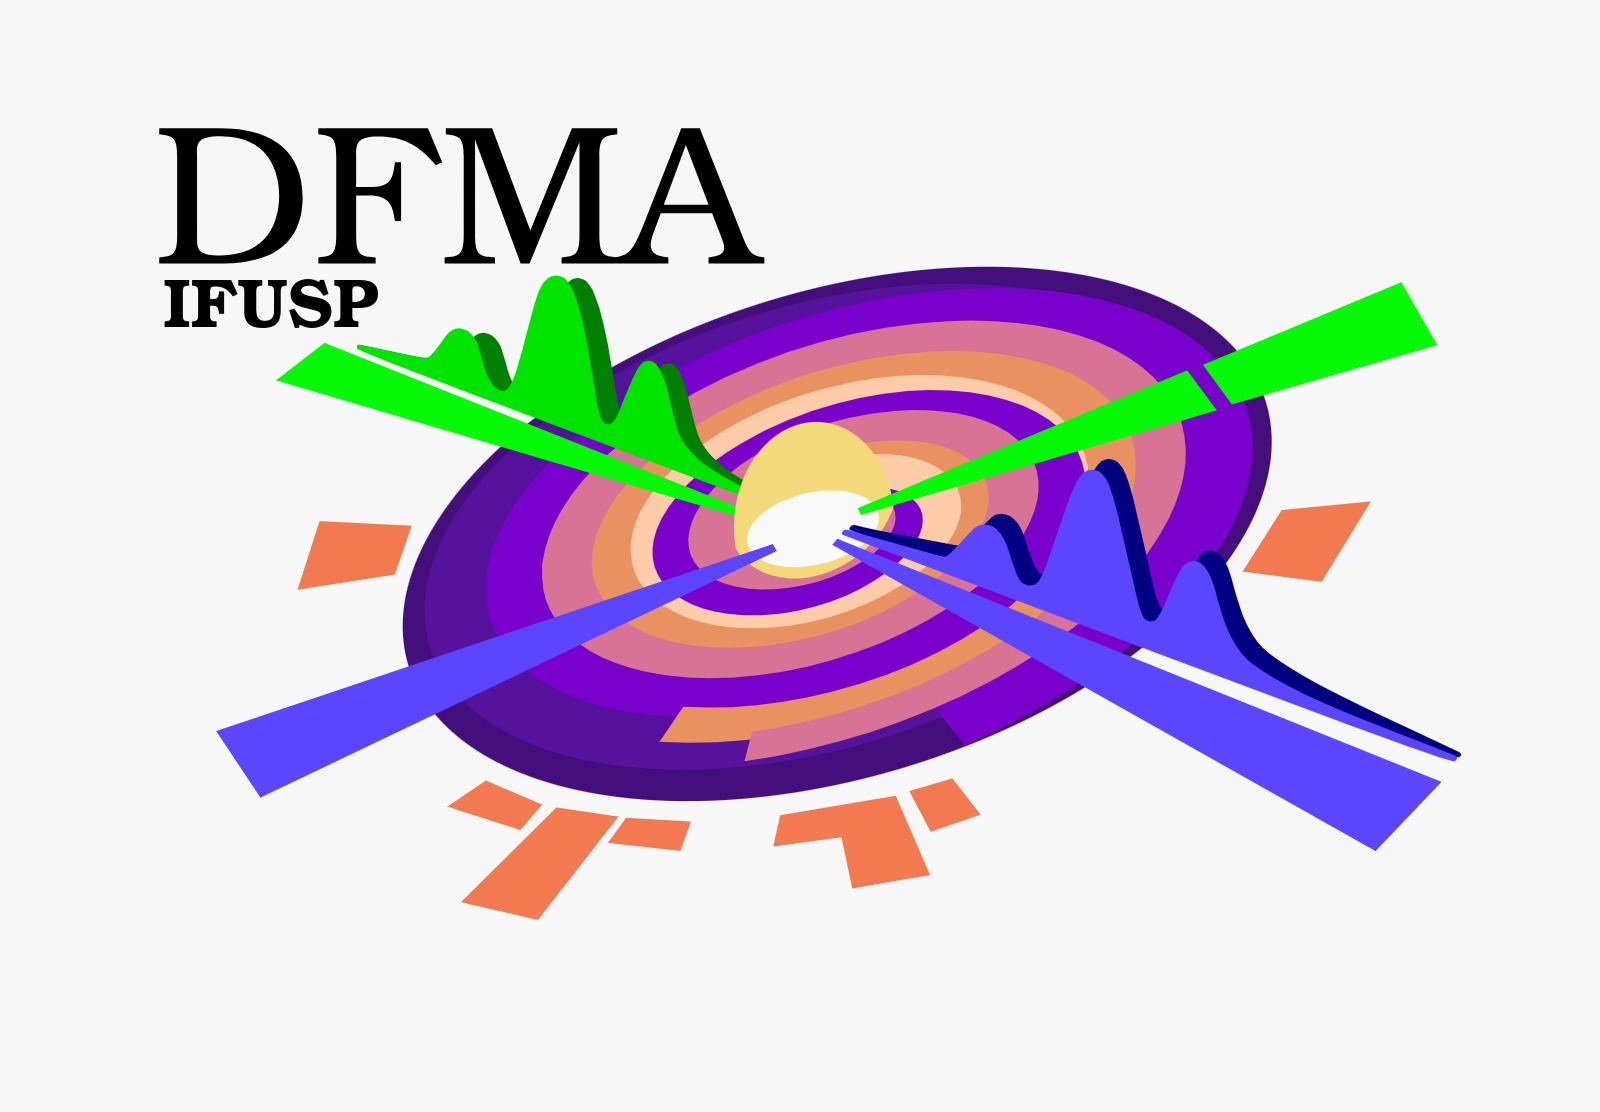
\includegraphics[width=\paperwidth,height=\paperheight]{agorameeting.jpg}%
  };
}

\begin{document}

\nocite{*}

% Slide de título
\begin{frame}
    \vspace{2cm}
    \titlepage%\centering%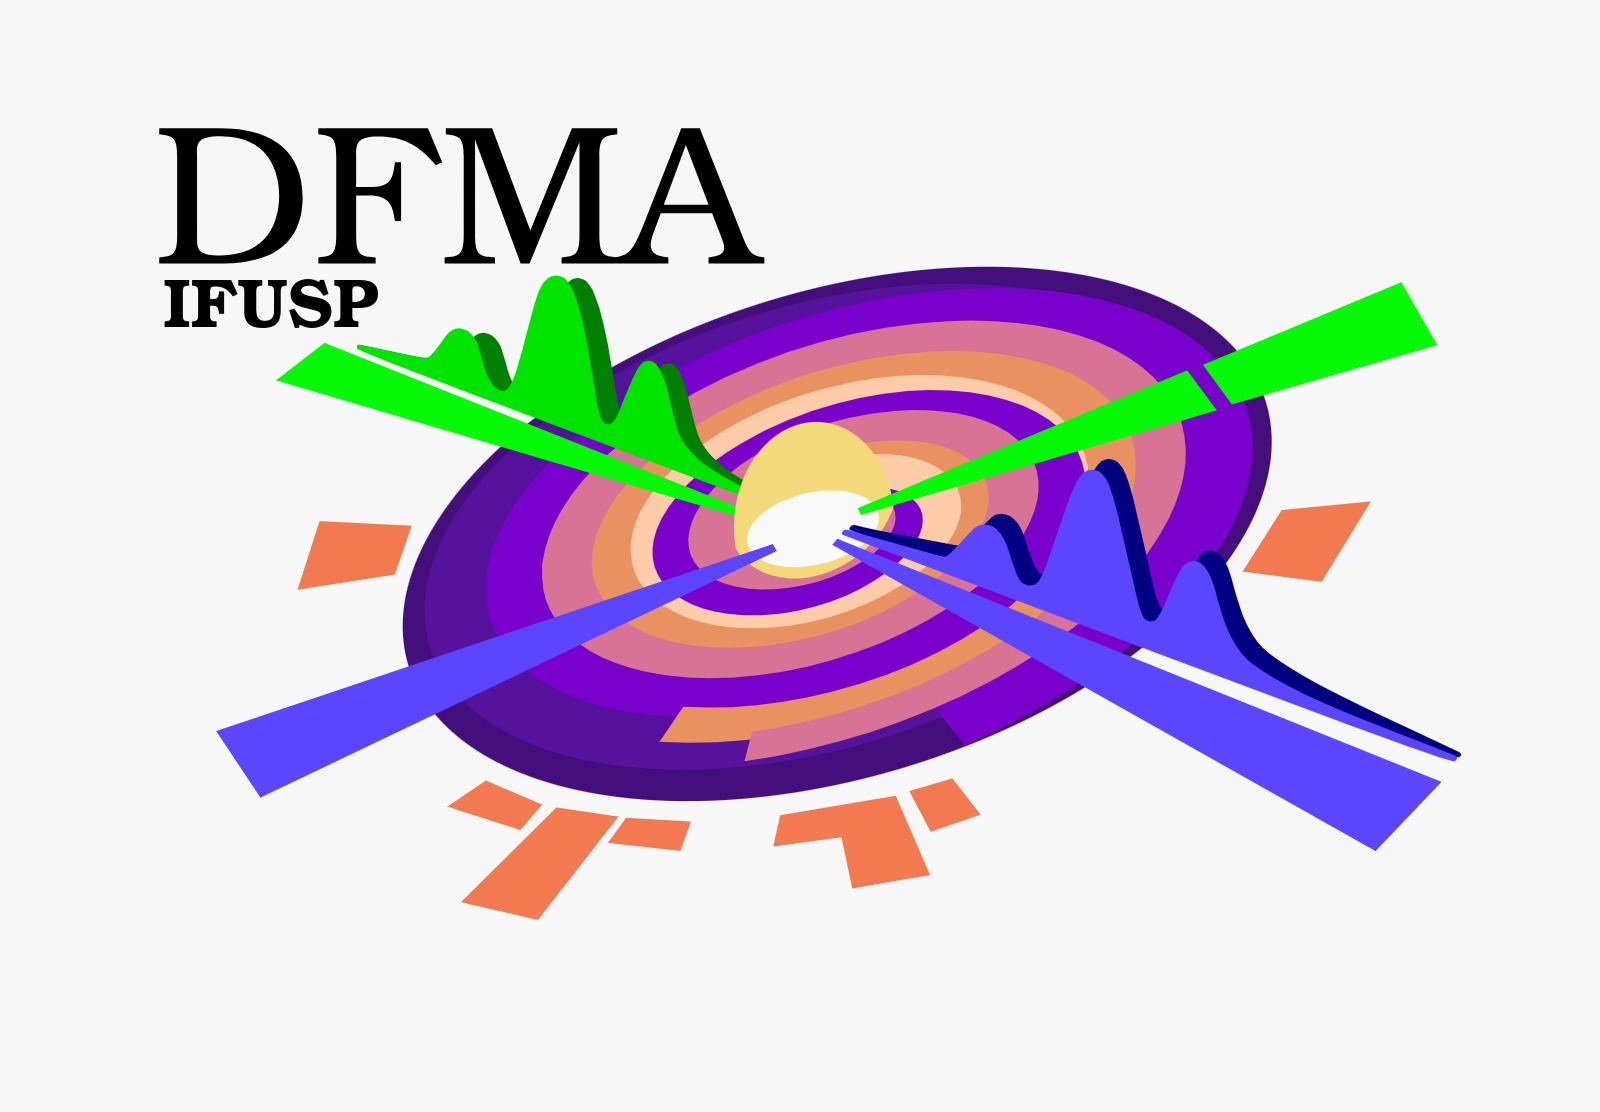
\includegraphics[width=0.8\textwidth]{agorameeting.jpg}
\end{frame}

% Slide de sumário
% \begin{frame}{Sumário}
%     \tableofcontents
% \end{frame}

% Seção: Introdução
\section{Motivation}
\begin{frame}{General Relativity}
    $$S_{\textnormal{EH}}=\frac{1}{2\kappa}\int\limits_M\dd[D]{x}\sqrt{\abs {g}}g^{ab}\tensor{R}{_c_a^c_b}$$\pause
    \begin{itemize}
        \item Non-polynomial $\rightarrow$ Hard to quantize.\pause
        \item Dimensionful coupling $\rightarrow$ Not perturbatively renormalizable.\pause
        \item Has diffeomorphism redundancies: $\phi_\ast\vb g\cong \vb g $.\pause
    \end{itemize}
    
    \vspace{2cm}

    We know how to quantize a class of theories with redundancies:
\end{frame}

\begin{frame}{Yang-Mills}
    $$S_{\textnormal{YM}}= \frac{1}{g^2}\int\limits_M\Tr\qty[\vb F\wedge \star \vb F],\ \ \ \vb F = \vb d\vb A+\wedgecomm{\vb A}{\vb A}$$
    \begin{itemize}
        \item Polynomial.\pause
        \item Dimensionless coupling $\rightarrow$ Renormalizable.\pause
        \item Has local Lie group-valued redundancies, $\vb A\cong U\qty(\vb A+\vb d)U^{-1}$.\pause
    \end{itemize}

    \vspace{1.5cm}

    It's possible to formulate GR as YM theory?

\end{frame}

\begin{frame}{Why $D=2+1$?}
    \begin{itemize}
        \item No local propagating modes:
        $$\textnormal{d.o.f.} = \frac12 D\qty(D-3)$$
    \end{itemize}
    Simpler but non-trivial toy model.
\end{frame}

\section{Reformulation}
\begin{frame}{Recover of polynomiality}
    \begin{itemize}
        \item Change of variables: $\vb g\rightarrow \begin{cases}\vb e^\mu,&\textnormal{ Vielbein} \\\boldsymbol\omega_{\alpha\beta},&\textnormal{ Spin connection} \end{cases}$\pause
        \item Relax torsionless condition $\rightarrow$ $\vb e^\mu$ and $\boldsymbol\omega_{\alpha\beta}$ are independent.\pause
    \end{itemize}

    \vspace{0.7cm}

    $$S_{\textnormal{EH}}= \frac{1}{2\kappa}\int\limits_M\star\vb R^{\alpha\beta}\wedge \vb e_\alpha\wedge \vb e_\beta\overset{D=3}{=}\frac{1}{2\kappa}\epsilon_{\alpha\beta\mu}\int\limits_M \vb R^{\alpha\beta}\wedge \vb e^\mu$$\pause
    
    \vspace{0.7cm}
    
    Can we write the integrand as a trace?
\end{frame}

\begin{frame}{Recover of dimensionless coupling constant}
    \begin{itemize}
        \item For $\mathfrak{iso}\qty(2,1)$: $$\Tr\qty[J_{\alpha\beta}P_\mu]=\frac{\lambda}{\kappa}\epsilon_{\alpha\beta\mu},\ \ \ \Tr\qty[P_\nu P_\mu]=0,\ \ \ \Tr\qty[J_{\alpha\beta}J_{\mu\nu}]=0$$\pause
        \item Dressing the fields with the algebra,
        $$S_{\textnormal{EH}}=\frac{1}{\lambda}\int\limits_M \Tr\qty[\vb R\wedge \vb e],\ \ \ \vb R=\frac12\vb R^{\alpha\beta}J_{\alpha\beta},\ \vb e=\vb e^\mu P_\mu$$\pause
    \end{itemize}

    \vspace{0.6cm}

    Not standard YM form...
\end{frame}

\section{Identification}

\begin{frame}{Chern-Simons}
    \begin{itemize}
        \item d.o.f. mismatch: $0$ v.s. $2N_c$\pause
        \item Available gauge theory with $0$ d.o.f.: Chern-Simons!
        $$S_{\textnormal{CS}}=\frac{1}{2\lambda}\int\limits_M\Tr\qty[\vb A \wedge \qty(\vb d{\vb A}+\frac13\wedgecomm{\vb A}{\vb A})]$$\pause
        \item Tentative: CS theory of ISO(2,1), $\vb A =\boldsymbol\omega+\vb e$,\pause
        $$S_{\textnormal{CS}}=\frac1\lambda\int\limits_M\expval{\vb e\ \wedgecomma\ \qty(\vb d{\boldsymbol\omega}+\frac12\wedgecomm{\boldsymbol\omega}{\boldsymbol\omega})}=S_{\textnormal{EH}}$$
    \end{itemize}
    Match!
\end{frame}

\section{Conclusions}

\begin{frame}{Conclusions}
    \begin{itemize}
        \item $2+1$ dimensional gravity is a CS gauge theory of ISO(2,1).\pause
        \item Opens path to quantization via well known CS methods.\pause
        \item Inclusion of cosmological constant change gauge group, $\begin{cases}\Lambda > 0: & \textnormal{SO}\qty(3,1),\ (\textnormal{dS})\\\Lambda < 0: & \textnormal{SO}\qty(2,2), \ (\textnormal{AdS})\end{cases}$\pause
        \item Offers a bridge between GR and usual gauge theory intuition.\pause
        \item Pose some suggestions about $D=3+1$.
    \end{itemize}
\end{frame}

\begin{frame}
    %\addtocounter{framenumber}{-1}
    \centering{Thank You!}
\end{frame}

\section{References}

\begin{frame}{References}
    \printbibliography
\end{frame}

\addtocounter{framenumber}{2000}

\end{document}